\documentclass%
%[handout]
{beamer}
% % % % % % % %
% % % % % % % %
% % % % % % % %
%IMPORTANT
%compiles with
%pdflatex -shell-escape
%IMPORTANT
% % % % % % % %
% % % % % % % %
% % % % % % % %
\mode<presentation>
{
\useinnertheme{rounded}
\useoutertheme{infolines}
\usecolortheme{orchid}
\usecolortheme{whale}
}

\usepackage[english]{babel}
\usepackage[latin1]{inputenc}
\usepackage[all,cmtip]{xy}
\usepackage{times}
\usepackage[T1]{fontenc}
\usepackage{../example-templates}
\usepackage{../pstricks-commands}

\usepackage{auto-pst-pdf}
\usepackage{pst-plot}
%\usepackage{pstricks-add}

% Or whatever. Note that the encoding and the font should match. If T1
% does not look nice, try deleting the line with the fontenc.


\graphicspath{{../../modules/}}

\newtheoremstyle{partialproof}{3pt}{3pt}{}{}{}{.}{.5em}{}
\theoremstyle{partialproof} \newtheorem{partialproof}[theorem]{Proof.}
%\DeclareMathOperator{\diff}{d}
\setbeamertemplate{navigation symbols}{}

\includeonlylecture{1}

\newcommand{\lect}[3]{
  \date{#1}
  \lecture[#1]{#2}{#3}
}

\setbeamertemplate{footline}
{
  \leavevmode%
  \hbox{%
  \begin{beamercolorbox}[wd=.333333\paperwidth,ht=2.25ex,dp=1ex,center]{author in head/foot}%
    \usebeamerfont{author in head/foot}\insertshortauthor
  \end{beamercolorbox}%
  \begin{beamercolorbox}[wd=.333333\paperwidth,ht=2.25ex,dp=1ex,center]{title in head/foot}%
    \usebeamerfont{title in head/foot}\insertshorttitle
  \end{beamercolorbox}%
  \begin{beamercolorbox}[wd=.333333\paperwidth,ht=2.25ex,dp=1ex,center]{date in head/foot}%
    \usebeamerfont{date in head/foot}\insertshortdate{}
  \end{beamercolorbox}}%
  \vskip0pt%
}

% If you have a file called "university-logo-filename.xxx", where xxx
% is a graphic format that can be processed by latex or pdflatex,
% resp., then you can add a logo as follows:

%\pgfdeclareimage[height=0.8cm]{logo}{bluelogo}
%\logo{\pgfuseimage{logo}}
\renewcommand{\Arcsin}{\arcsin}
\renewcommand{\Arccos}{\arccos}
\renewcommand{\Arctan}{\arctan}
\renewcommand{\Arccot}{\text{arccot\hspace{0.03cm}}}
\renewcommand{\Arcsec}{\text{arcsec\hspace{0.03cm}}}
\renewcommand{\Arccsc}{\text{arccsc\hspace{0.03cm}}}



\begin{document}

\AtBeginLecture{%

\title[\insertlecture]{FreeCalc}
\subtitle{\insertlecture}
\author[FreeCalc]{}
\institute[UMass Boston]{University of Massachusetts Boston}
\date{\insertshortlecture}
\begin{frame}
  \titlepage
\end{frame}
}%

% begin lecture
\lect{\today}{Sample}{1}{
%\begin{frame}
  \frametitle{Directional Derivatives}
\begin{itemize}
\item  Let $f \colon D \to \RR$, $P_0(\fcv{r}_0)$ in $D$, $\fcv{u}$ nonzero vector.
\item<2-> Let $L$ be line through $P_0$ with direction $\fcv{u}$, \alert<1->{oriented} by $\fcv{u}$.

\hfil{} $\fcv{r}\colon \RR \to L, \quad \fcv{r}(t) = \fcv{r}_0+t\fcv{u}$

\uncover<3->{
\begin{definition}[Covariant derivative $\nabla_{\fcv u} f$]
Let $\fcv u$ -nonzero vector. Define the covariant derivative $(\nabla_{\fcv{u}} f)$ via $(\nabla_{\fcv{u}} f) (P_0) = \lim_{t\to 0} \frac{f(\fcv{r}_0+t\fcv{u}) - f(\fcv{r}_0)}{t}$
\end{definition}
}
\item<4-> If $\fcv{r}$ is parametrized via arclength we have $|\fcv{u}|=1$
\uncover<5->{
\begin{definition}[Directional derivative]
Let $\fcv u$ be a unit vector. Define the directional derivative $D_{\fcv u} f$ via
$(D_{\fcv{u}} f)(P_0) = \lim_{t\to 0} \frac{f(\fcv{r}_0+t\fcv{u})-f(\fcv{r}_0)}{t}\; $.
\end{definition}
}
\item<6-> Define $(D_{\fcv{u}} f)(P_0)$ to be the instantaneous rate of change of $f$ along the line $L$.
\end{itemize}
\end{frame}
\begin{frame}
\frametitle{Partial Derivatives}
\begin{itemize} 
\item Let $f\colon D \to \RR$,  $P_0(x_0,y_0)$ inside $D$.
\item<2-> Consider the line $\fcv{r}(t) = \fcv{r}_0 + t\fcv {i} = \langle x_0+t, y_0 \rangle$.
\item<3-> Set $g(t) = f(\fcv{r}(t)) = f(x_0+t, y_0)$.
\item<4-> Then $(D_{\fcv{i}} f)(x_0,y_0) = \lim\limits_{t\to 0} \frac{g(t)-g(0)}{t}$
\begin{definition}[partial derivatives]
The partial derivatives $\frac{\partial}{\partial x} $, $\frac{\partial}{\partial y} $  of $f$ are defined as the directional derivatives of $f$ in the direction of the unit vector along the $x$, $y$ axes. 
\end{definition}
\end{itemize}
\end{frame}
\begin{frame}
  \frametitle{Example}
  Let $f(x,y) = y^2\ln{(2x+y)}- e^y$.

To compute $f_x$ \pause we treat $y$ as a constant.\pause
%
\begin{align*}
  f_x = \frac{\partial f}{\partial x} = & \frac{\partial(y^2\ln{(2x+y)}- e^y)}{\partial x} = \frac{\partial(y^2\ln{(2x+y)})}{\partial x} - \frac{\partial(e^y)}{\partial x} = \\
  %
  = & y^2 \frac{\partial(\ln{(2x+y)})}{\partial x} - 0 = y^2 \cdot \frac{1}{2x+y} \cdot \frac{\partial(2x+y)}{\partial x}= \frac{2y^2}{2x+y}\; .
\end{align*}

\pause To compute $f_y$ we treat $x$ as a constant:\pause
%
\begin{align*}
  f_y = \frac{\partial f}{\partial y} = & \frac{\partial(y^2\ln{(2x+y)}- e^y)}{\partial y} = \frac{\partial(y^2\ln{(2x+y)})}{\partial y} - \frac{\partial(e^y)}{\partial y} = \\
  %
  = & y^2 \frac{\partial(\ln{(2x+y)})}{\partial y} +\frac{\partial(y^2)}{\partial y} \ln{(2x+y)}
   - e^y = \\
   %
   = & y^2 \cdot \frac{1}{2x+y} \cdot \frac{\partial(2x+y)}{y} +2y\ln{(2x+y)} - e^y = \\
   %
   = & \frac{y^2}{2x+y} +2y\ln{(2x+y)} - e^y \; .
\end{align*}
\end{frame}

%\begin{frame}
\frametitle{Rate of Change}
\begin{itemize}
\item $O$: fixed point in space. Define $\alert<1->{f(P) = |OP|^2}$.
\item<2-> Question: How does $f$ change around a point $P_0$ in space? \uncover<3->{
$$\Delta f = f(P) - f(P_0)$$
}
\item<4->\alert<1->{Quantitative} question. What is the \alert<1->{rate of change} of $f$ at $P_0$?
\item<5-> The question is ambiguous: rate of change of $f$ with respect to what?
$$\text{ Rate of change } = \frac{f(P) - f(P_0)}{\textbf{?}}$$
\item<6-> Naive answer: with respect to \alert<1->{distance} from $P_0$:
$\frac{f(P) - f(P_0)}{|P_0P|}$.
\item<7-> Problem with naive answer: \alert<1->{the instantaneous rate of change may fail to exist:} $\lim_{P\to P_0} \frac{f(P)-f(P_0)}{|P_0P|}$.
\end{itemize}
\end{frame}
%\begin{frame}
  \frametitle{Rates of Change along Lines}
\begin{itemize}
\item Let $L$ be a line through $P_0(\fcv{r}_0)$.
\begin{center}  How does $f(\fcv{r}) = |\fcv{r}|^2$ change \alert<1->{along $L$}?  
\end{center}
\item<2-> Let $\fcv{r} : \RR \to L$: smooth parametrization of $L$, $\fcv{r}(0) = \fcv{r}_0$
$$g\colon \RR \to \RR, \quad g(t) = f(\fcv{r}(t))$$
\begin{center}
Rate of change of $f$ along $L$ = rate of change of $g$.
\end{center}
\item<3-> With respect to $t$:
$$\lim_{t\to 0} \frac{f(\fcv{r}(t))-f(\fcv{r}(0))}{t} =\lim_{t\to 0} \frac{g(t)-g(0)}{t} = g'(0)$$
\item<4-> Still ambiguous: depends on the parametrization $\fcv{r}$.
\item<5-> To resolve that use arclength parametrization.
\item<6-> Almost solves the problem: orientation still matters.
\end{itemize}
\end{frame}


%\begin{frame}
  \frametitle{Continuity of vector fields}
\begin{itemize}
\item Recall that a vector field is a function 
\[
\begin{array}{rcl}
\fcv{F}\colon D &\to& \RR^2 \\ 
\fcv{F}(x,y) &=& F_1(x,y) \fcv{i} + F_2(x,y) \fcv{j} 
\end{array}
\]
\item<2-> $F_1, F_2$ are two-variable functions with scalar output.
\item<3-> We have already defined the notion of continuity of $F_1$ and $F_2$.
\item<4-> We define $\fcv{F}$ to be continuous if $ F_1$ $F_2$ are continuous.
\end{itemize}

\end{frame}
%\begin{frame}
\begin{example}[of continuous vector field]
\begin{columns} 
\column{0.4\textwidth}
\psset{xunit=1.75cm, yunit=1.75cm}
\begin{pspicture}(-1.25, -1.25)(1.25,1.25)
\fcBoundingBox{-1.25}{-1.25}{1.25}{1.25}
\fcAxesStandard{-1}{-1}{1}{1}
\fcVectorField[arrows=->, linecolor=blue]{iterationsX=9, iterationsY=9, Delta=0.25, startX=-1 , startY=-1}{y 3 div x 3 div}
\end{pspicture}
\column{0.6\textwidth}
Discuss the continuity of the following vector field.
$$\textbf{F}(x,y) =\frac{y}{2}  \textbf{i} -\frac{x}{2}\textbf{j}\quad .$$
\end{columns}

\uncover<2->{Then 

$$F_1(x,y) = \frac{y}{2} \quad , \quad F_2(x,y) = -\frac{x}{2} $$}

\uncover<3->{We have that $y, -x$ are two-variable polynomials} \uncover<4->{$\Longrightarrow$ $F_1$ and $F_2$ are continuous} \uncover<5->{$\Longrightarrow$ the vector field is continuous.}
\end{example}
\end{frame}
%\begin{frame}
\frametitle{Side Limits and Directional Limits}
\begin{itemize}
\item Directional limits in dimension 1 are equal to the left or right hand limits (depending on the direction of the vector).
\item<2-> Directional limits are therefore the natural analog of 1-dim side limits.
\item<3-> Similarities b-n side and directional limits.
\begin{itemize}
\item<3-> Single variable functions: limit exists $\Longrightarrow$ side limits exist, have the same value.
\item<4-> Multivariable functions: limit exists $\Longrightarrow$ directional limits exist, have the same value.
\item<5-> Singe variable functions: side limits are different $\Longrightarrow$ limit does not exist.
\item<6-> Multivariable functions: directional limits have different values $\Longrightarrow$ limit does not exist.
\end{itemize}
\item<7-> Differences b-n side and directional limits.
\begin{itemize}
\item<7-> Single variable functions: Side limits are equal $\Longrightarrow$ limit exists.
\item<8-> Multivariable functions: even if all directional limits have the same value the limit does not necessarily exist.
\end{itemize}
  
\end{itemize}

\end{frame}
%\begin{frame}
\begin{example}[\uncover<12->{All directional limits exist, limit doesn't}]    %
\[
\lim\limits_{(x,y) \to (0,0)} \frac{xy^2}{x^2+y^4}
\]
\uncover<2->{
Along $y=mx$, we have
\[
\frac{xy^2}{x^2+y^4} = \uncover<3->{\frac{m^2 x^3}{x^2+m^4x^4}} \uncover<4->{=  \frac{m^2 x}{1+m^2x^4}} \uncover<5->{\alert<12>{ \to  0 \text{ as } x \to 0}.}
\]
\uncover<6->{For the direction $x=0$, $y=m$ direct computation shows that the directional limit is again $0$.} 
\uncover<7->{Therefore all directional limits exist and are equal.}
}

\uncover<8->{However, along $x=y^2$:}
\[
\uncover<8->{\frac{xy^2}{x^2+y^4} =}\uncover<9->{ \frac{y^4}{y^4+y^4} = }\uncover<10->{ \frac{1}{2} }\uncover<11->{\alert<12>{\to  \frac{1}{2} \text{ as } x \to 0}}
\]
\uncover<12->{\alert<12>{Therefore $\lim\limits_{(x,y) \to (0,0)} \frac{xy^2}{x^2+y^4}$ does not exist.}}
\end{example}
\end{frame}
%\begin{frame}
\frametitle{Limits along paths}
\begin{definition}
\begin{itemize}
\item<1-> Let $f: D\to \mathbb R$, where $D$ is a region in the plane;
\item<2-> let  $f$ be defined near point $P$ with position vector $\fcv p$.
\item<3-> Let $\fcv r(t)=(x(t), y(t))$, $t\in I$ be a continuous path such that:
\begin{itemize}
\item<3-> $0$ is in $I$, $\fcv{r}(0) = \fcv p$;
\item<4-> $\fcv{r}$ is continuous at $0$;
\item<5-> $\fcv{r}(t)$ lies in $D$ for $t\neq 0$
\end{itemize}
\end{itemize}
\uncover<6->{ 
We say that the one-variable limit
\[
\lim\limits_{t\to 0} f(\fcv{r}(t))
\]
is the limit of $f$ along the path $\fcv r(t)$.
}
\end{definition}
\end{frame}
\begin{frame}
\begin{theorem}
If the limit $\lim\limits_{Q\to P}f(Q) $ exists, then every path limit exists and all path limits are equal.
\end{theorem}
\begin{itemize}
\item<2-> If we pick our path to be of the form $\fcv{r}(t) = \fcv{r}_0+t\fcv{u}$, we see that the directional limit is a special case of the path limit.
\end{itemize}
\end{frame}

%\begin{frame}
\begin{example}
\[\lim_{(x,y) \to (0,0)} \frac{x^2y}{x^2+y^2}
\]
\begin{itemize}
\item<2-> $f$ is not defined at $P_0(0,0)$;
\item<3-> Even if it were, the actual value might be different from the limit.
\end{itemize}
\uncover<4->{Recall polar coordinates: \alert<9,10>{ $x=r\cos\theta$, $y =r \sin\theta$}. \alert<8>{ We have that \alert<5,6>{$(x,y) \to (0,0)$ if an only if $\uncover<-5>{\textbf{?}} \uncover<6->{r\to 0}$  \alert<9,10>{ in polar coordinates}.}}}
\[
\begin{array}{rcl}
\uncover<7->{ \displaystyle \lim\limits_{\alert<8>{(x,y) \to (0,0)}} \alert<9,10>{ \frac{x^2y}{x^2+y^2} } &\alert<9,10>{=}& \displaystyle  \lim\limits_{\alert<8>{r\to 0}}  \uncover<-9>{\alert<9>{\textbf{?}}} \uncover<10->{\alert<10>{\frac{\alert<11>{ r^2}\cos^2\theta r\sin\theta}{\alert<11>{r^2}}}}} \\
\uncover<11->{&\alert<0>{=}&\displaystyle \lim\limits_{r\to 0}\phantom{\textbf{?}} \alert<12>{r\cos^2{\theta}\sin\theta}}\\
\uncover<15->{&\alert<0>{=}&0}
\end{array}	
\]
\uncover<15->{For the last equality, we use the squeeze theorem:} 
\uncover<12->{$\uncover<14->{0=} \uncover<13->{\lim\limits_{r\to 0} } -r \leq \uncover<13->{ \lim \limits_{r \to 0}} \alert<12>{ r\cos^2{\theta}\sin\theta } \leq \uncover<13->{\lim\limits_{r\to 0}}  r \uncover<14->{=0.}$}
\end{example}
\end{frame}
%\begin{frame}
If $\fcv r =\langle a,b \rangle$ is a vector, by $f(\fcv r) $ we understand $f(a,b) $ (i.e., define $f(\fcv r)$ via the vector-point identification).
\begin{definition}
\begin{itemize}
\item<2-> Let $f: D\to \mathbb R$, where $D$ is a region in the plane;
\item<3-> let  $f$ be defined near $P$ with position vector $\fcv r$; $f$ is not necessarily defined at $P$;
\item<4-> let $\fcv u$ be an arbitrary vector.
\end{itemize}
\uncover<5->{ 
We say that the one-variable limit
\[
\lim\limits_{t\to 0} f(\fcv{r}+t\fcv{u})
\]
is the limit of $f$ along the direction $\fcv u$.
}
\end{definition}
\uncover<6->{
\begin{theorem}
If the limit $\lim\limits_{Q\to P}f(Q) $ exists, then every directional limit $\lim\limits_{t\to 0 } f(\fcv r+t\fcv u ) $ exists and all directional limits are equal.
\end{theorem}
}
\end{frame}

%\begin{frame}
\begin{example}[Limit may fail to exist]
\[
\lim_{(x,y) \to (0,0)} \frac{xy}{x^2+y^2}
\]

\uncover<2->{Let $\fcv u= ( 1,m)$ and use directional limit along $\fcv u$:}

\centering
$\begin{array}{rcl}
\uncover<2->{ \displaystyle\lim\limits_{t\to 0} f(t\fcv{u}) &=&\displaystyle\lim\limits_{t\to 0} f(t( 1,m))=\displaystyle\lim\limits_{t\to 0} f(t, tm)}\\
\uncover<3->{&=&\displaystyle\lim_{t\to 0}\frac{m \alert<4>{t^2}}{\alert<4>{t^2}+m^2\alert<4>{t^2}}}\\
\uncover<4->{&=& \displaystyle\frac{m}{1+m^2}}\quad.
\end{array}
$
\flushleft

\uncover<5->{Directional limit depends on $m$ $\Rightarrow$} \uncover<6->{directional limit is not the same for all values of $\textbf{u}$} \uncover<7->{$\Rightarrow$ the multivariable limit does not exist.}

\uncover<8->{If we'd used polar coordinates, we would had obtained:

\centering
{
$\displaystyle
\uncover<8->{\alert<8,9>{ \frac{xy}{x^2+y^2} =}} \uncover<9->{ \alert<9>{ \cos \theta \sin\theta}}
$
}
}
\flushleft

\uncover<10->{This expression depends only on $\theta$; as $r\to 0$ permits arbitrary behavior of $\theta$, we'd had guessed correctly that the limit doesn't exist.}

\end{example}
\end{frame}


%\begin{frame}
\frametitle{Multivariable Limits}
\begin{itemize}
\item Let $f\colon D \to \RR$, where $D$ a subset of the plane. 
\item<2-> Let $P_0$ be point in plane such that:
\begin{itemize}
\item<2-> \alert<5>{$f$ is defined arbitrarily close to $P_0$};
\item<3-> \alert<6>{$f$ is not necessarily defined at $P_0$}.
\end{itemize}
\item<4-> For example,
\[ 
\begin{array}{rcl}
\displaystyle f \colon  \RR^2\setminus \{ P_0(0,0)\} &\to&\displaystyle  \RR \\
\displaystyle f(x,y)& =& \displaystyle \frac{x^2y}{\alert<6> {x^2+y^2}}
\end{array}
\]
\begin{itemize}
\item<4-> \alert<5>{is defined arbitrarily close to $(0,0)$};
\item<4-> \alert<6>{and is not defined at $P_0(0,0)$}.
\end{itemize}
\item<7-> Question: What happens to $f(Q)$ as $Q$ gets closer to $P_0$?
\end{itemize}
\end{frame}
%\begin{frame}
\frametitle{Numerical Exploration of Limits - Example}
\begin{example}

$$f(x,y) = \frac{x^2y}{x^2+y^2}$$
$$f(Q) \to ? \text{ as } Q\to  P_0(0,0)$$

\uncover<2->{
Numerical approach:
\[
\begin{array}{r|rcl}
Q_1(0.1,0.1)  & f(Q_1) &=& f(0.1,0.1) \simeq 0.05\\
\uncover<3->{Q_2(0.01,-0.02) & f(Q_2) &=& f(0.01,-0.02) \simeq -0.004}\\
\uncover<4->{Q_3(-0.003,0.001) & f(Q_3) &=& f(-0.003,0.001) \simeq 0.0009}
\end{array}
\]
}
\uncover<5->{ 
Numerical data suggests $f(Q)$ approaches $0$ as $Q \to P_0(0,0)$.
}
\end{example}
\end{frame}

%\begin{frame}
\frametitle{Definition of Multivariable Limit}
\begin{itemize}
\item Let $f\colon D \to \RR$, with $D$ a subset of the plane.
\item Let $P_0$ be a point in the plane such that:
\begin{itemize}
\item $f$ is defined arbitrarily close to $P_0$;
\item $f$ is not necessarily defined at $P_0$.
\end{itemize}
\uncover<2->{
\begin{definition}
$L$ is \alertNoH{1-}{the limit of $f$ at $P_0$} if we can keep the values of $f(Q)$ as close to $L$ as we want by keeping $Q$ close enough to $P_0$, but not equal to $P_0$. \uncover<3->{We write:
\[
\begin{array}{rcll}
L &=& \lim\limits_{Q\to P_0} f(Q) &\text{ or } \\
L &=& \lim\limits_{(x,y) \to (x_0,y_0)} f(x,y)
\end{array}
\]
}
\end{definition}
}
\item<4-> As usual, we extend the definition to allow $L=\infty$. By convention, if $M>N$, we say that $M$ is closer to $\infty$ than $N$.
\item<5-> If the limit $L$ exists, it is unique.
\end{itemize}
\end{frame}


%\begin{frame}
\begin{pspicture}(-1, -1)(2,2)
\fcBoundingBox{-3}{-3}{4}{4}%
%\multido{\na=1+1}{10}{%
%\only<\na>{\renewcommand{\fcScreen}{[-1 1 -0.5 -0.31 \na \space 1 sub mul add] 0}%
\fcStartIIIdScene%
\fcSurfaceInScene[iterationsU=5, iterationsV=3]{0}{-1}{240}{1}{[u cos u sin v]}{}%
\fcFinishIIIdScene%
%}%
%} %
\end{pspicture}
%\uncover<10>{}
\end{frame}

%\input{../../modules/TESTING/surfaces-test-twisted-moebius-band}
%\begin{frame}
\begin{pspicture}(-1, -1)(2,2)
\fcBoundingBox{-3}{-3}{4}{4} %
\fcStartIIIdScene%
\fcSurfaceInScene[
iterationsU=33
, 
iterationsV=5
]{0}{-1}{360}{1}{%
[10 dict begin
/R 2 def
/r {0.8 v mul} def
/theta u def
/phi {u 0.5 mul} def
/A {phi cos r mul R add} def
theta cos A mul theta sin A mul phi sin r mul
end %
]%
}{}%
%\fcLineIIIdInScene[linewidth=2, linecolor=cyan]{[-1 -1 -1]}{[1 1 1]}
\fcFinishIIIdScene[true] %
\end{pspicture}
\end{frame}

%\input{../../modules/TESTING/rotation-along-helix}
%\begin{frame}
\frametitle{Application}
$$|\fcv{r}|' = \frac{\fcv{r} \cdot \fcv{r}'}{|\fcv{r}|}$$

\begin{itemize}
\item Suppose a point has a trajectory on a sphere with center at origin. Therefore:
\[
\begin{array}{rcl}
\uncover<2->{ |\fcv{r}(t)|& = &\text{constant }\\}
\uncover<3->{|\fcv{r}(t)|'&=& 0 \\}
\uncover<4->{\fcv{r}(t)\cdot \fcv{r}'(t)&=& 0 }
\end{array}
\]
\item<5-> In other words, $\fcv r(t)=\text{constant}$ implies $\fcv{r}(t) \bot \fcv{r}'(t)$.
\item<6-> Velocity  $\bot$ Position  $\Longleftrightarrow$ Velocity vector $\fcv{r}'(t)$ tangent to sphere.
\item<7-> What can we say about constant acceleration?
$$\fcv{r}\cdot \fcv{r}'\equiv 0 \Longrightarrow [\fcv{r}\cdot \fcv{r}']' = 0 \Longleftrightarrow \fcv{r}'\cdot \fcv{r}'+\fcv{r}\cdot \fcv{r}'' = 0 \Longrightarrow \fcv{r}\cdot \fcv{r}'' = -|\fcv{r}'|^2 \leq 0$$
Acceleration vector $\fcv{r}''$ points inside the sphere.
\end{itemize}
\end{frame}
%\begin{frame}
\begin{example}
\begin{columns}
\column{0.4\textwidth}
\begin{pspicture}(-2, -2)(2, 2)
\fcBoundingBox{-2.4}{-1.1}{2.4}{2.4}
\fcAxesIIId{3}{3}{2}

\pstVerb{
6 dict begin 
/phi  {t 3 mul} def 
/theta {t 2 mul} def 
/R 2 def 
/r 0.2 def 
/xyRad {phi sin r mul R add} def 
/trefoil {[theta cos xyRad mul theta sin xyRad mul phi cos r mul ]} def
}
\fcCurveIIId[linecolor=red, plotpoints=500]{0}{10 }{trefoil}
\fcCurveIIId[linecolor=red, plotpoints=500]{49}{195 }{trefoil}
\fcCurveIIId[linecolor=red, plotpoints=500]{205}{315 }{trefoil}
\fcCurveIIId[linecolor=red, plotpoints=500]{325 }{400}{trefoil}
\pstVerb{end}
\end{pspicture}
\column{0.6\textwidth}
Compute the curvature of the torus (trefoil) curve 

$
\begin{array}{rcl}
x&=& \left(R+r\sin \left(3t\right)\right) \cos (2t) \\
y&=& (R+r\sin \left( 3t \right) \sin 2t \\
z&=& r\cos (3t) 
\end{array}
$
\end{columns}
\end{example}

\end{frame}
%\input{../../modules/parametric-curves/curvature-example-torus-sphere-twisted-meridian}
%\begin{frame}
\begin{example}
\begin{columns}
\column{0.4\textwidth}
\begin{pspicture}(-2, -2)(2, 2)
\fcBoundingBox{-2.4}{-1.1}{2.4}{2.4}
\fcAxesIIId{3}{3}{2}

\pstVerb{
4 dict begin 
/phi  {t } def 
/theta {t 0.2 mul} def 
/R 1 def 
/twistedMeridian {[theta cos phi sin mul R mul theta sin phi sin mul R mul phi cos R mul ]} def
}
\fcCurveIIId[linecolor=red, plotpoints=500]{0 }{180}{twistedMeridian}
\fcLineIIId{[0 0 0]}{[3 0 0]}
\pstVerb{end}
\end{pspicture}
\column{0.6\textwidth}
Find $\fcv r''(t)= \langle x(t), y(t),z(t) \rangle$, where
$
\begin{array}{rcl}
x(t)&=& \rho \sin (at)\cos (bt) \\
y(t)&=& \rho\sin(at)\sin (bt) \\
z(t)&=& \rho\cos (at) 
\end{array}
$

A river is flowing from north to south in the northern hemisphere. In which direction is the force caused by the earth's rotation (Coriolis force) pushing the river's water?
\end{columns}
\end{example}

\end{frame}

%\begin{frame}
\frametitle{Curvature}
\begin{itemize}
\item \underline{Question}: How can we \emph{measure} how bent a curve is?
\item \underline{Answer}: Measure change in tangent direction with respect to arclength.
\end{itemize}
 \begin{itemize}
\item $\fcv{p}=\fcv{p}(s)$: parametrization by arclength of smooth curve $C$;
\item $\fcv{v}$: fixed direction (unit vector);
\item $\fcv{T}(s)$: unit tangent vector;
\item $\alpha(s)$: angle between $\fcv{T}(s)$ and $\fcv{v}$;
\item We define the \emph{curvature} of $C$ at $\fcv{p}(s)$ to be
\[\kappa(s) = \left| \alpha'(s) \right|\; .
\]
\item Simpler formulas:
\[\kappa(s) = | \fcv{T}'(s) | = \left| \frac{d\fcv{T}}{ds}\right| \; .
\]
\item $\fcv{r}=\fcv{r}(t)$: smooth parametrization, not necessary by arclength.
\[\kappa(t) = \frac{|\fcv{T}'(t)|}{|\fcv{r}'(t)|} = \frac{|\fcv{r}''(t) \times \fcv{r}'(t)|}
{|\fcv{r}'(t)|^3}\; .
\]
\end{itemize} 
\end{frame}
%\begin{frame}
Notation: $\fcv T$- unit tangent vector, $\fcv r$- position vector, $\kappa$-curvature.
\begin{example}
Compute the curvature of $\fcv{r}(t) = ( \cos{t}, \sin{t}, t)$.
\begin{columns}
\column{0.5\textwidth}
$\begin{array}{rcl}
\uncover<2->{\alert<2,3> {\fcv{r}'(t)}}& \uncover<2->{\alert<2,3>{=}}&\uncover<3->{\alert<3>{\displaystyle ( -\sin{t}, \cos{t}, 1 ) }}\\
\uncover<4->{\alert<4,5>{ |\fcv{r}'(t)|}} & \uncover<4->{\alert<4,5>{=}}&\uncover<5->{\alert<5>{ \displaystyle \sqrt{2}}}\\
\uncover<6->{\alert<6,7>{\fcv{T}(t)}} &\uncover<6->{\alert<6,7>{=}} &\displaystyle \uncover<7->{\alert<7>{ \frac{1}{\sqrt{2}} ( -\sin{t}, \cos{t}, 1 ) }}\\
\end{array}
$
\column{0.5\textwidth}
$\begin{array}{rcl}
\uncover<8->{\alert<8,9>{\fcv{T}'(t)}} &\uncover<8->{\alert<8,9>{=}}& \uncover<9->{\alert<9>{\frac{1}{\sqrt{2}}( -\cos{t}, -\sin{t}, 0 ) }}\\
\uncover<10->{\alert<10,11>{|\fcv{T}'|}}&\uncover<10->{\alert<10,11>{=}}&\uncover<11->{\alert<11>{ \frac{1}{\sqrt{2}}}} \\
\uncover<12->{\alert<12,13>{ \kappa(t)}} &\uncover<12->{\alert<12,13>{=}}& \uncover<13->{\alert<13>{ \frac{|\fcv{T}'(t)|}{|\fcv{r}'(t)|} =
\frac{1}{2}}} \quad .\\
\end{array}
$
\end{columns}

\uncover<14->{Alternatively: }
\[
\begin{array}{rcl}
\uncover<14->{\alert<14,15>{\fcv{r}''}} &\uncover<14->{\alert<14,15>{=}}& \uncover<15->{\alert<15>{ ( -\cos{t}, -\sin{t}, 0 )}} \\
\uncover<16->{\alert<16,17>{ \fcv{r}'' \times \fcv{r}'}} &\uncover<16->{\alert<16,17>{=}}&\uncover<17->{\alert<17>{\displaystyle \left|
\begin{array}{ccc}
\fcv{i} & \fcv{j} & \fcv{k} \\
-\cos{t}&  -\sin{t}&  0 \\
-\sin{t}& \cos{t}& 1
\end{array}
\right| = -\sin{t} \, \fcv{i} +
\cos{t}\, \fcv{j} -\fcv{k}}} \\~\\
\uncover<18->{\alert<18,19>{
\kappa(t) }}&\uncover<18->{\alert<18,19>{=}}&\uncover<19->{\alert<19>{ \displaystyle \frac{|\fcv{r}''(t) \times \fcv{r}'(t)|} {|\fcv{r}'(t)|^3} =\frac{\sqrt{2}}{(\sqrt{2})^3} = \frac{1}{2}\; .}}
\end{array}
\]
\end{example}
\end{frame}


%\begin{frame}
\begin{example}
\begin{columns}
\column{0.35\textwidth}
\uncover<2->{
\begin{pspicture}(-1.7,-1.5)(1.8,3)%
\tiny%
\pstVerb{5 dict begin /pi 3.141592654 def}%
\renewcommand{\fcScreen}{[-1 1 -7] 0}
\fcBoundingBox{-1.7}{-1.5}{1.7}{3}%
\fcAxesIIId{2}{2}{10}%
\fcCurveIIId[plotpoints=500, linecolor=red]{0}{720}{[t cos t sin t 180 div pi mul]}%
\pstVerb{end}%
\end{pspicture}
}
\column{0.65\textwidth}
Let $\fcv{r}(t) = ( \cos{t}, \sin{t}, t)$  \uncover<2->{(the curve is called a \alertNoH{2}{helix} - (not a spiral) ).}
\begin{itemize}
\item \alertNoH{1}{Do you know the name of this curve?}
\item Find the arclength function.
\item Find the length of the segment of the curve given by $t\in [0,2\pi]$.
\end{itemize}
\end{columns}


\[
\begin{array}{rcl}
\uncover<3->{\fcv{r}'(t) &=& ( -\sin{t}, \cos{t}, 1 ) \\}
\uncover<4->{\fcv{r}'(t)| &= &\sqrt{2}\quad .}\\
\uncover<5->{
L(t) &=&\displaystyle \int_0^t |\fcv{r}'(\tau)| \diff \tau \\
\uncover<6->{& =& t\sqrt{2} \quad  .}
}
\end{array}
\]

\end{example}
\end{frame}


%\begin{frame}
  \frametitle{Example}
  
  \begin{itemize}
    \item $\fcv{r}(t) = \langle \cos{t}, \sin{t}, t\rangle \Longrightarrow \fcv{r}'(t) = \langle -\sin{t}, \cos{t}, 1 \rangle \Longrightarrow|\fcv{r}'(t)| = \sqrt{2}$;
%
$$\fcv{T}(t) = \frac{1}{\sqrt{2}}
\langle -\sin{t}, \cos{t}, 1 \rangle
\Longrightarrow
\fcv{T}'(t) = \frac{1}{\sqrt{2}}
\langle -\cos{t}, -\sin{t}, 0 \rangle
\Longrightarrow $$
$$|\fcv{T}'|=\frac{1}{\sqrt{2}}$$
 %
 \item Curvature:
%
$$\kappa(t) = \frac{|\fcv{T}'(t)|}{|\fcv{r}'(t)|} =
\frac{1}{2}\; .$$ 
  \end{itemize}

Alternatively: $\fcv{r}''= \langle -\cos{t}, -\sin{t}, 0 \rangle$,
%
$$\fcv{r}'' \times \fcv{r}' = \left|
\begin{array}{ccc}
\fcv{i} & \fcv{j} & \fcv{k} \\
-\cos{t}&  -\sin{t}&  0 \\
-\sin{t}& \cos{t}& 1
\end{array}
\right| = -\sin{t} \, \fcv{i} +
\cos{t}\, \fcv{j} -\fcv{k} $$
%
$$\kappa(t) =
\frac{|\fcv{r}''(t) \times \fcv{r}'(t)|}
{|\fcv{r}'(t)|^3} =
\frac{\sqrt{2}}{(\sqrt{2})^3} = \frac{1}{2}\; .$$

\end{frame}
%\begin{frame}
\begin{example}
Let $\fcv r(t)$ be the coordinate curves for the spherical coordinates, i.e., let
\[
\begin{array}{rcl}
\fcv{e}_\rho(t)&=& \alert<2,3>{ \langle t\sin \phi \cos \theta, t\sin \phi \sin \theta, t\cos \phi \rangle }\\
\fcv{e}_\phi(t)&=& \alert<4,5>{ \langle \rho\sin t \cos \theta, \rho\sin t \sin \theta, \rho\cos t \rangle }\\
\fcv{e}_\theta(t)& =& \alert<6,7>{\langle \rho\sin\phi \cos{t}, \rho\sin\phi \sin{t}, \rho\cos\phi\rangle }\\
\end{array}
\]
where $\rho$, $\phi$, $\theta$ are regarded as constants and $t$ as the curve parameter. Find $\fcv {e}_\rho'(t)$, $\fcv e_\phi'(t)$, $\fcv e_\theta'(t)$. Compute $ (\fcv e_\rho '(\rho) \times \fcv e_{\theta}'(\theta) )\cdot \fcv e_{\phi}'(\phi)$.

\[
\begin{array}{rcl}
\uncover<2->{\alert<2,3,8>{ \fcv{e}_\rho '(t)} &\alert<2,3>{=}&\uncover<3->{\alert<3,8>{ \langle \sin \phi \cos \theta, \sin \phi\sin \theta, \cos \phi \rangle }}\\}
\uncover<4->{\alert<4,5,9>{\fcv e_{\phi}'(t)} &\alert<4,5>{=}&\uncover<5->{ \alert<5,9>{ \langle \rho\cos t \cos\theta, \rho\cos t \sin\theta, -\rho\sin t \rangle}} }\\
\uncover<6->{\alert<6,7,10>{\fcv e_{\theta}'(t)} &\alert<6,7>{=}&\uncover<7->{ \alert<7,10>{ \langle -\rho\sin \phi \sin t, \rho\sin \phi \cos t, 0 \rangle}} }\\
\uncover<8->{
(\fcv{e}_{\rho}'(\rho) \times \fcv{e}_{\phi}'(\phi)) \cdot \fcv{e}_{\theta}'(\theta) &=&\alert<11,12>{ \left| \begin{array}{ccc}
\alert<8>{ \sin \phi \cos \theta }& \alert<8>{\sin \phi \sin\theta }&  \alert<8>{\cos\phi} \\
\alert<9>{\rho \cos \phi \cos \theta }&\alert<9>{ \rho \cos \phi\sin \theta }&\alert<9>{ -\rho \sin \phi} \\
\alert<10>{-\rho \sin \phi\sin \theta }&\alert<10>{ \rho \sin \phi \cos \theta }&\alert<10>{0}
\end{array}\right|} \\}
\uncover<11->{&\alert<11,12>{=}&\uncover<12->{\alert<12>{\rho^2\sin\phi }}}
\end{array}
\]
\end{example}
\end{frame}
%\begin{frame}
\begin{itemize}
\item An analytical description is technically best, but not easy to interpret.
\item If output is a scalar, where does the function attain its extreme values (maxima, minima)?  
\item How do values change for nearby points - are they decreasing, increasing, how fast?
\item We will learn to decode this information from the analytical descriptions.
\item Even so, ``a picture is worth a thousand words (and, say, 10 f-las)''.
\end{itemize}
\end{frame}

\begin{frame}
\begin{center}
\psset{xunit=1cm,yunit=1cm}
\begin{pspicture}(-3,-3)(3,5.5)

\psset{Beta=15}
\psplotThreeD[plotstyle=line,drawStyle=xLines,yPlotpoints=50,xPlotpoints=50,linewidth=0.3pt, linecolor=blue](-4,4)(-4,4){ x 3 exp x y 4 exp mul add x 5 div sub 10 mul 2.729 x dup mul y dup mul add neg exp mul 2.729 x 1.225 sub dup mul y dup mul add neg exp add}
\pstThreeDCoor[xMin=-1,xMax=5,yMin=-1,yMax=5,zMin=-1,zMax=5]
\rput[t](-3,5.3){Graph of a scalar function.}
\end{pspicture}
\end{center}

\end{frame}

\begin{frame}\frametitle{Graph of a function}
\begin{itemize}
\item For one variable function, $y=f(x)$, the graph of $f$ is a set of points in $\RR^2$: the set of points $(x,y)$ such that $y=f(x)$.
\item Example: if $f(x) = x^2$, then  $(3,9)$ is on the graph, because $9=3^2$, but $(2,5)$ is not because $5 \neq 2^2$.
\item We can extend this graphical representation for functions with two dimensional input and one dimensional (scalar) output. 
\item The \emph{graph} of the function $f\colon D \to \RR$, where $D$ is a region in $\RR^2$, is the set of points $P(x,y,z)$ in $\RR^3$ whose coordinates satisfy the condition 
\[
z=f(x,y)\quad .
\]
\item For example, the graph of $f(x,y) = 2x-y+3$ is the set
\[
\{ (x,y,z) \, | \, z= 2x-y+3\} \Longrightarrow \text{ plane } 2x-y-z+3=0 \; .
\]

\end{itemize}

 



\end{frame}


%\begin{frame}

\begin{pspicture}(-1, -1)(2,2)
\fcBoundingBox{-1}{-1}{2}{2}
\pstVerb{ 
[] [] \fcAreEqual == 
[1] [2] \fcAreEqual == 
[1] [1] \fcAreEqual ==
[[1 0] 1] [[1 0] 1] \fcAreEqual ==
[[1 1] 1] [[1 0] 1] \fcAreEqual ==
[[1 [5 0]] 1] [[1 [5 0]] 1] \fcAreEqual ==
[[1 [5 1]] 1] [[1 [5 0]] 1] \fcAreEqual ==
}
\end{pspicture}
\end{frame}
%\begin{frame}
We have the ellipsoid 
\[
\frac{x^2}{a^2}+\frac{y^2}{b^2}+\frac{z^2}{c^2}= 1.
\]
We are seeking to project it orthographically onto the plane 
\[
px+qy+rz=s.
\]
The direction in which our ``orthographic eye'' is looking is $\fcv n= (p,q,r)$.
\end{frame}
\begin{frame}
\begin{pspicture}(-0.2,-0.2)(3,3)
\fcStartIIIdScene
\fcEllipsoid{1 2 3}
\fcFinishIIIdScene
\end{pspicture}
\end{frame}

%\begin{frame}
\frametitle{Continuity}
\begin{definition}
Suppose
\begin{itemize}
\item $\fcv{r}$ is defined at $t_0$
\item<2-> $\lim\limits_{t\to t_0} \fcv{r}(t)$ exists.
\end{itemize}
\uncover<3->{
Then we say that $\fcv{r} \colon [a,b] \to \RR^3$ is continuous at $t_0$ if
\[
\lim_{t\to t_0} \fcv{r}(t) = \fcv{r}(t_0)\quad .
\]
}
\end{definition}
\begin{observation}
$\fcv{r}(t) = ( x(t), y(t), z(t) )$ is continuous at $t_0$ $\Longleftrightarrow$ $x(t), y(t), z(t) $ are all continuous at $t_0$.

\end{observation}


\end{frame}

%
\begin{frame}
\frametitle{Limits}
\begin{definition}
We say that $$\lim_{t\to a} \fcv{r}(t) = \fcv{u}$$ if \alertNoH{4}{ by selecting that } $t\neq a$ be close enough to $a$ \alertNoH{5}{we can guarantee that $\fcv{r}(t)$} \alertNoH{3}{is as close to $\fcv{u}$ as we want}.

\medskip

\uncover<2->{In strict mathematical language: $\lim_{t\to a} \fcv{r}(t) = \fcv{u}$ if \alertNoH{3}{for every $\varepsilon >0$} \alertNoH{4}{there exists $\delta>0$} \alertNoH{5}{ such that for all $t$ with $0<|t-a|<\delta $} \alertNoH{3}{we have that $| \fcv r(t)-u|<\varepsilon $}.}
\end{definition}
\end{frame}

\begin{frame}
\begin{itemize}
\item We define the ``postman distance'' between $(x_1,y_1,z_1)$ and $(x_2, y_2, z_2)$ to be the number $\max(|x_1-x_2|, |y_1-y_2|, |z_1-z_2|) $.
\item<2-> Two points in Euclidean distance are close if and only if they are close in ``postman distance''.
\item<3-> Unlike higher dimensions, in dimension 1 postman distance coincides with Euclidean distance.
\item<4-> Let $\fcv{r}(t) = ( x(t), y(t), z(t) )$ and $\fcv{u}=( u_1,u_2,u_3)$.
\item<5-> Then
\[
\lim_{t\to a} \fcv{r}(t) = \fcv{u} \Longleftrightarrow
\left|
\begin{array}{l}
\lim\limits_{t\to a} x(t) = u_1\\
\lim\limits_{t\to a} y(t) = u_2\\
\lim\limits_{t\to a} z(t) = u_3\\
\end{array}
\right.\quad .
\]
\end{itemize}
\end{frame}

%\makeatletter
\psset{xunit=1.1cm, yunit=1.1cm}
\begin{pspicture}(-2.2,-3.9)(2.345,3.234)
%\fcSet{shiftX=-3.1, shiftY=-2.8}
\fcBoundingBox{-2}{-2}{2}{2}
\fcLine{[0 0 ]}{[0 1]}
\fcLine{[0 0 ]}{[1 0]}
\psline(0, 0)(0,-1)
\psline(0.5, 0)(-1,0)

\end{pspicture}
\makeatother
\begin{frame}
\end{frame}
%\begin{frame}
\begin{pspicture}(-1, -1)(2,2)
\fcBoundingBox{-1}{-1}{2}{2}
\fcSurfaceDirectDraw{iterationsX=10, iterationsY=10, Delta=1}{-90}{-1}{90}{1}{[u cos u sin v]}
\end{pspicture}
\begin{pspicture}(-1, -1)(2,2)
\fcBoundingBox{-3}{-3}{4}{4} %
\renewcommand{\fcScreen}{[-1 1 -0.8] 0}
\multido{\na=1+1}{10}{%
\only<\na->{\renewcommand{\fcScreen}{[-1 1 -0.5 -0.3 \na \space mul add] 0}
}
} %
\fcStartIIIdScene %
\fcSurfaceInScene[iterationsU=13, iterationsV=4]{0}{-1}{360}{1}{[u cos u sin v]}
%\fcSurfaceInScene[iterationsU=1, iterationsV=2]{-1}{-1}{0}{0}{ [u  v add 2 u mul v sub  v u add]} %
\fcFinishIIIdScene %
\end{pspicture}
%\uncover<10>{}
\end{frame}

%\begin{frame}
\begin{pspicture}(-2,-2)(2,2)
%\pstVerb{[1 5 6]  \fcArrayToStack stack}

\pstVerb{[1 2 3] [4 5 6] 7 \fcProjectOntoPlane \fcArrayToStack stack}

%\pstVerb{[1 2 3] 5 \fcVectorTimesScalar \fcArrayToStack stack}
%\pscircle*[fillcolor=white, linecolor=red](! \fcProjectOriginOnPlane{1}{1}{1}{1}){0.07}


\end{pspicture}
\end{frame}
%

\begin{frame}
\frametitle{Constant Coordinate Sets}
\begin{columns}[T]
\column{0.55\textwidth}
\psset{xunit=2.5cm, yunit=2.5cm}
\begin{pspicture}(-1.2, -1.8)(2.5,1.6)
\tiny%
\renewcommand{\fcScreen}{[-3 -1 -1] 0}%
\fcBoundingBox{-1.2}{-1.2}{2}{2}%
\fcLineIIId[arrows=->]{[0 0 0]}{[1.5 0 0]}%
\fcLineIIId[arrows=->]{[0 0 0]}{[0 1.5 0]}%
\fcLineIIId[arrows=->]{[0 0 0]}{[0 0 1.5]}%
\pstVerb{3 dict begin%
/xPoint 0.5 sqrt def%
/yPoint 0.5 sqrt def%
/zPoint 1 def%
}%
\multido{\na=1+1}{6}{\only<\na-7>{\pstVerb{%
/xPoint 1 \na\space 1 sub 10 div sub def%
/yPoint xPoint def%
}}%
\uncover<\na-6>{%
\fcDotIIId[linecolor=gray]{[1 \na\space 1 sub 10 div sub dup 1]}%
}%
}%
\multido{\na=8+1}{6}{\only<\na-14>{\pstVerb{%
\na\space 7 sub 12 mul dup
/xPoint exch cos def%
/yPoint exch sin def%
}}%
\uncover<\na-13>{%
\fcDotIIId[linecolor=gray]{[\na\space 7 sub 12 mul dup cos exch sin 1]}%
}%
}%
\multido{\na=15+1}{6}{\only<\na-21>{\pstVerb{%
/zPoint \na\space 15 sub -0.2 mul 1.2 add def%
}}%
\uncover<\na-20>{%
\fcDotIIId[linecolor=gray]{[xPoint yPoint \na\space 15 sub -0.2 mul 1.2 add]}%
}%
}%
\fcPerpendicularIIId[linestyle=dashed]{[xPoint yPoint zPoint]}{[0 0 1]}{0.2}%
\fcLineIIId{[0 0 0]}{[xPoint yPoint zPoint]}%
\fcPerpendicularIIId{[xPoint yPoint zPoint]}{[xPoint yPoint 0]}{0.2}%
\fcPutIIId[bl]{[xPoint yPoint zPoint]}{$~~P(x, y, z)$}
\fcPutIIId[tl]{[xPoint yPoint 0]}{$~~Q$}
\fcPerpendicularIIId[linestyle=dashed]{[xPoint yPoint 0]}{[1 0 0]}{0.2}%
\fcPerpendicularIIId[linestyle=dashed]{[xPoint yPoint 0]}{[0 1 0]}{0.2}%
\fcLineIIId{[0 0 0]}{[xPoint yPoint 0]}%
\fcPutIIId[r]{[xPoint 2 div 0 0]}{$x~~$}
\fcPutIIId[b]{[0 yPoint 2 div 0]}{$y$}
\fcPutIIId[r]{[0 0 zPoint 2 div]}{$z~~$}
\fcDotIIId{[xPoint yPoint zPoint]}%
\fcDotIIId{[xPoint yPoint 0]}%
\fcPutIIId[tr]{[xPoint 2 div yPoint 2 div 0]}{$r$}%
\fcAngleIIId[arrows=->, linecolor=red]{[1 0 0]}{[xPoint yPoint 0]}{0.3}%
\fcPutIIId[t]{[xPoint xPoint mul yPoint yPoint mul add sqrt dup xPoint exch div 0.4 mul exch yPoint exch div 2 div 0.4 mul 0]}{$\theta$}%
\uncover<7>{%
\fcLineIIId[arrows=->, linecolor=red]{[0 0 1]}{[1.4 1.4 1]}%
}%
\uncover<14>{%
\fcCurveIIId{-180}{180}{[t cos t sin 1]}%
}%
\uncover<21>{%
\fcLineIIId[linecolor=red]{[0.5 sqrt dup -0.2]}{[0.5 sqrt dup 1.5]}%
}%
\uncover<23>{%
\fcSurfaceDirectDraw[linecolor=red]{iterationsX=11, iterationsY=11}{0}{-0.4}{180}{1}{[u cos u sin  v]}%
}%
\uncover<25>{%
\fcSurfaceDirectDraw[linecolor=red]{iterationsX=11, iterationsY=17}{0}{-0.4}{1.6}{1.2}{[u u v]}%
}%
\uncover<27>{%
\fcSurfaceDirectDraw[linecolor=red]{iterationsX=11, iterationsY=13}{0}{-180}{1.2}{180}{[v sin u mul v cos u mul 1]}%
}%
\pstVerb{end}%
\end{pspicture}
\column{0.45\textwidth}
What curve is traced when:
\begin{itemize}
\item \alert<1-7>{keep $\theta, z$ constant, let $r $ vary:} \uncover<7->{\alert<7>{horizontal ray;}}
\item \alert<8-14>{keep $r, z$ constant, let $\theta$ vary:} \uncover<14->{\alert<14>{horizontal circle;}}
\item \alert<15-21>{keep $r, \theta$ constant, let $z$ vary:} \uncover<21->{\alert<21>{ vertical line.}}
\end{itemize}

What surface is traced when:
\begin{itemize}
\item \alert<22,23>{keep $r$ constant, let $\theta, z$ vary:} \uncover<23->{\alert<23>{vertical cylinder;}}
\item \alert<24,25>{keep $\theta$ constant, let $r,z$ vary:} \uncover<25->{\alert<25>{vertical half plane;}}
\item \alert<26,27>{keep $z$ constant, let $r,\theta$ vary:} \uncover<27->{\alert<27>{horizontal plane.}}
\end{itemize}
\uncover<15>{}
\end{columns}
\end{frame}

%\begin{frame}
\frametitle{A motivating example}
What does the graph $\Gamma$ of $g$ look like?
\[
g(x,y) =x^2+2y^2\quad .
\]

\begin{pspicture}(-2,-2)(2,2)
\psC

\end{pspicture}

\begin{itemize}
\item The graph $\Gamma$ is the set of points $P(x,y,z)$ in $\RR^3$ such that $z=x^2+2y^2$. The set is not a plane: what does it look like?
\item To answer look at sections. Use imaginary CT scan to cut the graph; assemble resulting sections into a graph.
\item Cut by vertical planes parallel to the $Oyz-$plane.
\item Suppose cutting plane has equation $x=a$, where $a$-constant. Intersection with cutting plane is given by points:
\[
\{(a, y, z)\quad \text{where } z=a^2+2y^2)\}
\]
\item These cross-sections are parabolas lying inside the plane $x=a$ with vertices at $(a,0,a^2)$. The vertex rises as $a$ gets away from $0$.
\item When we intersect $\Gamma$ with the plane $x=a$ we treat $x$ as a constant and study the function $y\to z=g(a,y) = a^2+2y^2$.
\end{itemize}



Similarly, if we cut by planes $y=a$ we get partial
functions $x\to x^2+2a^2$, whose graphs are also
parabolas. Each such a parabola is now situated in the
vertical plane $y=a$. Hence vertical sections are
parabolas, with vertices rising as
we move farther away from the coordinate planes.

To get horizontal sections we have to
keep constant not an input variable, but the output
variable, $z$. Intersecting the graph of $g$ with
the plane $z=a$ we get a curve of equations $x^2+2y^2=a$,
$z=a$. For $a<0$ the intersection is empty, for $a=0$ it
consists of a single point, $(x,y,z) = (0,0,0)$, and for
$a>0$, the intersection is an ellipse in the plane $z=a$.

The \emph{level curve} corresponding to $z=a$ is the curve
$g(x,y)=a$ in the domain of $g$, with a label $a$ to
indicate the level of the output corresponding to
that level curve. Note that the level curve is not the
intersection of the graph of $g$ with the plane $z=a$;
instead, it is the projection of that intersection onto
the plane $Oxy$, where the domain of $g$ resides.

You should be familiarized with level curves if
you have ever seen a topographic map or if you
opened the newspaper at the weather section. What are the
functions in those cases?

\end{frame}


\subsection{Level sets}
The examples considered in the previous sections were all
examples of functions with scalar output and a two
dimensional input. Their graphs lived in
$\RR^3 = \RR^{2+1}$, with the 2 coming from the dimension
of the input and the 1 from the dimension of the output.
If we wanted to extend that graphic construction to
functions depending on three scalar variables,
we'd need $3+1=4$ dimensions for the graphs, and that
is momentarily impossible. The rescue comes from the
second graphical representation, using level sets,
because the level sets (with appropriate labeling of
the level) can be represented in a space with dimension
equal to the dimension of the input space.


For example, let $f(x,y,z) = ax+by-z$. The graph is the
quadruple $(x,y,z,w)$ in $\RR^4$ such that
$w = ax+by-z$, and we can't yet represent that
graphically. But the level set $f(x,y,z) = d$ is the
surface $ax+by-z = d$ in $\RR^3$, and that surface is a
plane. Level sets corresponding to equidistant values
$d_1$, $d_2$, and $d_3$ of the output are parallel
planes of equations
%
\begin{align*}
  \mathcal{P}_1 = f^{-1}(d_1) & \colon \; ax+by-z = d_1\\
  %
  \mathcal{P}_2 = f^{-1}(d_2) & \colon \; ax+by-z = d_2\\
  %
  \mathcal{P}_3 = f^{-1}(d_3) & \colon \; ax+by-z = d_3
\end{align*}
%
and these planes are also equidistant.

The following remark will play a very important role in
understanding surfaces in space.

\begin{remark}{\rm The level set $f(x,y,z)=0$ for the
function
%
$$f(x,y,z) = ax+by-z+d$$
%
is the same as the graph
of the function $g(x,y) = ax+by+c$.
}\end{remark}

We will see that while graph surfaces can always be
represented as level surfaces, the converse is not true:
level surfaces can't always be represented as graph
surfaces. However, we'll show that under some reasonable
assumptions, level surfaces can \emph{locally} be
described as graph surfaces. An illuminating example is
that of a sphere (centered at the origin): it is the
level surface of $f(x,y,z) = x^2+y^2+z^2$, but it can't
be globally represented as a graph surface. Try and see
what goes wrong!


%\begin{frame}
Looking for $t $ such that 
\[
\begin{array}{rcl}
\displaystyle\langle \mathbf{v}+t \mathbf{n}, \mathbf{n}\rangle  &=&\displaystyle d\\
\displaystyle t&=&\displaystyle \frac{d-\langle\mathbf{v},\mathbf{n} \rangle}{\langle\mathbf{n}, \mathbf{n} \rangle}
\end{array}
\]
\end{frame}

\begin{frame}
Helicoid.
\begin{pspicture}(-2,-2)(2,2)
\fcAxesIIId{2}{2}{2}
\fcCurveIIId[linecolor=red, plotpoints=100]{0}{1440}{t cos t sin t 360 div }
\end{pspicture}

\end{frame}
\begin{frame}
\uncover<11>{}
\begin{pspicture}(-2,-2)(2,2)

\only<1>{\renewcommand{\fcScreen}{[-1 1 0.25] -1}
\fcAxesIIId{2}{2}{2}
\fcCurveIIId[linecolor=red, plotpoints=100]{0}{1440}{t cos t sin t 360 div}
}
\only<2>{\renewcommand{\fcScreen}{[-1 1 0.25] -1.1}
\fcAxesIIId{2}{2}{2}
\fcCurveIIId[linecolor=red, plotpoints=100]{0}{1440}{t cos t sin t 360 div}
}
\only<3>{\renewcommand{\fcScreen}{[-1 1 0.25] -1.2}
\fcAxesIIId{2}{2}{2}
\fcCurveIIId[linecolor=red, plotpoints=100]{0}{1440}{t cos t sin t 360 div}
}
\only<4>{\renewcommand{\fcScreen}{[-1 1 0.25] -1.3}
\fcAxesIIId{2}{2}{2}
\fcCurveIIId[linecolor=red, plotpoints=100]{0}{1440}{t cos t sin t 360 div}
}
\only<5>{\renewcommand{\fcScreen}{[-1 1 0.25] -1.4}
\fcAxesIIId{2}{2}{2}
\fcCurveIIId[linecolor=red, plotpoints=100]{0}{1440}{t cos t sin t 360 div}
}
\only<6>{\renewcommand{\fcScreen}{[-1 1 0.25] -1.5}
\fcAxesIIId{2}{2}{2}
\fcCurveIIId[linecolor=red, plotpoints=100]{0}{1440}{t cos t sin t 360 div}
}
\only<7>{\renewcommand{\fcScreen}{[-1 1 0.25] -1.6}
\fcAxesIIId{2}{2}{2}
\fcCurveIIId[linecolor=red, plotpoints=100]{0}{1440}{t cos t sin t 360 div}
}
\only<8>{\renewcommand{\fcScreen}{[-1 1 0.25] -1.7}
\fcAxesIIId{2}{2}{2}
\fcCurveIIId[linecolor=red, plotpoints=100]{0}{1440}{t cos t sin t 360 div}
}
\only<9>{\renewcommand{\fcScreen}{[-1 1 0.25] -1.8}
\fcAxesIIId{2}{2}{2}
\fcCurveIIId[linecolor=red, plotpoints=100]{0}{1440}{t cos t sin t 360 div}
}
\only<10>{\renewcommand{\fcScreen}{[-1 1 0.25] -1.9}
\fcAxesIIId{2}{2}{2}
\fcCurveIIId[linecolor=red, plotpoints=100]{0}{1440}{t cos t sin t 360 div}
}
\only<11>{\renewcommand{\fcScreen}{[-1 1 0.25] -2}
\fcAxesIIId{2}{2}{2}
\fcCurveIIId[linecolor=red, plotpoints=100]{0}{1440}{t cos t sin t 360 div}
}
\end{pspicture}
\end{frame}

\begin{frame}
\uncover<11>{}
\begin{pspicture}(-2,-2)(2,2)

\only<1>{\renewcommand{\fcScreen}{[-1 1 0] -1}
\fcAxesIIId{2}{2}{2}
\fcCurveIIId[linecolor=red, plotpoints=100]{0}{1440}{t cos t sin t 360 div}
}
\only<2>{\renewcommand{\fcScreen}{[-1 1 0.1] -1}
\fcAxesIIId{2}{2}{2}
\fcCurveIIId[linecolor=red, plotpoints=100]{0}{1440}{t cos t sin t 360 div}
}
\only<3>{\renewcommand{\fcScreen}{[-1 1 0.2] -1}
\fcAxesIIId{2}{2}{2}
\fcCurveIIId[linecolor=red, plotpoints=100]{0}{1440}{t cos t sin t 360 div}
}
\only<4>{\renewcommand{\fcScreen}{[-1 1 0.3] -1}
\fcAxesIIId{2}{2}{2}
\fcCurveIIId[linecolor=red, plotpoints=100]{0}{1440}{t cos t sin t 360 div}
}
\only<5>{\renewcommand{\fcScreen}{[-1 1 0.4] -1}
\fcAxesIIId{2}{2}{2}
\fcCurveIIId[linecolor=red, plotpoints=100]{0}{1440}{t cos t sin t 360 div}
}
\only<6>{\renewcommand{\fcScreen}{[-1 1 0.5] -1}
\fcAxesIIId{2}{2}{2}
\fcCurveIIId[linecolor=red, plotpoints=100]{0}{1440}{t cos t sin t 360 div}
}
\only<7>{\renewcommand{\fcScreen}{[-1 1 0.6] -1}
\fcAxesIIId{2}{2}{2}
\fcCurveIIId[linecolor=red, plotpoints=100]{0}{1440}{t cos t sin t 360 div}
}
\only<8>{\renewcommand{\fcScreen}{[-1 1 0.7] -1}
\fcAxesIIId{2}{2}{2}
\fcCurveIIId[linecolor=red, plotpoints=100]{0}{1440}{t cos t sin t 360 div}
}
\only<9>{\renewcommand{\fcScreen}{[-1 1 0.8] -1}
\fcAxesIIId{2}{2}{2}
\fcCurveIIId[linecolor=red, plotpoints=100]{0}{1440}{t cos t sin t 360 div}
}
\only<10>{\renewcommand{\fcScreen}{[-1 1 0.9] -1}
\fcAxesIIId{2}{2}{2}
\fcCurveIIId[linecolor=red, plotpoints=100]{0}{1440}{t cos t sin t 360 div}
}
\only<11>{\renewcommand{\fcScreen}{[-1 1 1] -1}
\fcAxesIIId{2}{2}{2}
\fcCurveIIId[linecolor=red, plotpoints=100]{0}{1440}{t cos t sin t 360 div}
}
\end{pspicture}
\end{frame}


\begin{pspicture}(-2,-2)(2,2)
%\pstVerb{[1 5 6]  \fcArrayToStack stack}

%\pstVerb{[1 2 3] [4 5 6] 7 \fcProjectOntoPlane \fcArrayToStack stack}

%\pstVerb{[1 2 3] [4 5 6] 7 \fcProjectOntoPlane ==}
%\pstVerb{[1 1 0] [1 1 1] \fcVectorCrossVector ==}
%\pscircle*[fillcolor=white, linecolor=red](! \fcProjectOriginOnPlane{1}{1}{1}{1}){0.07}
%\parametricplot{0}{360}{t sin t cos}
\end{pspicture}


%\begin{frame}
\begin{pspicture}(-2,-2)(2,2)
\fcAxesIIId{2}{2}{2}
\end{pspicture}
\end{frame}
%

\begin{frame}


\psset{xunit=1cm, yunit=1cm}
\stripPoints{\psxunit}
\stripPoints{\psyunit}

\begin{pspicture}(0,0)(1,1)
\psline(0,1)(7,1)
\fcLine{[0 0]}{[7 0]}
\pstVerb{%
\expandbefore \fcCurve{0}{360}{[t cos t sin]} %
newpath %
0 0 moveto %
100 100 lineto %
stroke %
} %
%\fcLine{[0 0]}{[100 -200]}
%\fcLine{[0 0]}{[100 90]}
%\fcLine{[0 0]}{[100 -90]}
\end{pspicture}
%\begin{pspicture}(-1,-1)(1,1)
%\end{pspicture}

\end{frame}
%\begin{frame}
We have the ellipsoid 
\[
\frac{x^2}{a^2}+\frac{y^2}{b^2}+\frac{z^2}{c^2}= 1.
\]
We are seeking to project it orthographically onto the plane 
\[
px+qy+rz=s.
\]
The direction in which our ``orthographic eye'' is looking is $\fcv n= (p,q,r)$.
\end{frame}
\begin{frame}
\begin{pspicture}(-0.2,-0.2)(3,3)
\fcStartIIIdScene
\fcEllipsoid{1 2 3}
\fcFinishIIIdScene
\end{pspicture}
\end{frame}
%\begin{frame}

\psset{xunit=0.4cm, yunit=0.4cm}
\begin{pspicture}(-5,-5)(5,5)
\fcAxesStandard{-5}{-5}{5}{5}
\fcVectorField[linecolor=blue, arrows=->]{-5}{-5}{11}{11}{1}{1 dict begin /r x x mul y y mul add sqrt def  r 0 eq {0 0} {-1 y mul r div  x r div} ifelse end}
\end{pspicture}

\end{frame}




%\begin{frame}
\frametitle{Quadratic surfaces} 
\begin{itemize}
\item The level sets for second degree polynomial functions
\[
f(x,y,z) = \alert<2>{Ax^2+By^2+Cz^2+Dxy+Exz+Fyz} +Gx+Hy+Iz+J.
\]
are called \alert<1->{quadratic surfaces}.
\item<2-> At least one of the \alert<2>{second-degree terms} is required to be non-zero.
\item<3-> The coefficients are allowed to be zero.
\end{itemize}
\end{frame}

\begin{frame}
\frametitle{Canonical forms of quadratic surfaces.}
Through rigid motions (translations and rotations) a quadratic surface can be reduced to one of the two canonical forms.
\begin{itemize}
\item<2-> 
\[  
\begin{array}{rcl} 
Ax^2+By^2+Cz^2+D &=& 0,\\
\uncover<handout: 0|5->{\alert<5>{A(-x)^2+B(-y)^2+C(-z)^2+D} &\alert<5>{=}& \alert<5>{0} ,} 
\end{array} 
\] 
$(A, B, C)\neq (0,0,0)$. 
\uncover<4->{ These quadratics posses central symmetry:} \uncover<5->{\alert<5>{if $(x,y,z)$ belongs to the surface, so does $(-x,-y,-z)$.}}
\item<3-> 
\[
\alert<6>{ Ax^2+By^2+Iz=0,}
\] 
$(A, B, C)\neq (0,0,0)$, $\alert<6>{I\neq 0}$.
\uncover<6->{These quadratics do not posses central symmetry.}
\end{itemize}

\uncover<7->{
The canonical forms above are in addition split into sub-forms depending on the sign of $A, B, C, D, I$. 
}

\end{frame}
%
\begin{frame}
\frametitle{$Ax^2+By^2+Cz^2+D=0$, $A>0, B>0, C>0, D>0$}
Consider the surface 
$\mathcal C =\{(x,y,z) |Ax^2+By^2+Cz^2+D=0 \}$.

\begin{itemize}
\item Let $A>0, B>0, C>0, D>0$.
\item<2-> Then the surface is the empty set.
\item<3-> Example: 
\[
x^2+2y^2+3z^2+4=0.
\]
\end{itemize}
\vskip 10cm

\end{frame}
%
\begin{frame}
\frametitle{$Ax^2+By^2+Cz^2+D=0$, $A>0, B>0, C>0, D>0$}
Consider the surface 
$\mathcal C =\{(x,y,z) |Ax^2+By^2+Cz^2+D=0 \}$.


\begin{columns} 
\column{0.4\textwidth}
\psset{xunit=1cm, yunit=1cm}
\begin{pspicture}(-2,-2)(2, 2)
\fcAxesIIId{2}{2}{2}
\end{pspicture}

\column{0.6\textwidth}
\begin{itemize}
\item Let $A>0, B>0, C>0$, $D<0$.
\item<2-> Set $A=\frac{1}{a^2}$, $B=\frac{1}{b^2}$, $C=\frac{1}{c^2}$, $D=-d^2$.
\item<3-> Surface becomes:
$\left\{(x,y,z)|\left(\frac{x}{a}\right)^2+\left(\frac{y}{b}\right)^2+\left(\frac{y}{z}\right)^2= d^2\right\}$.
\item<4-> We illustrate the theory on the example:
$\frac{1}{2}x^2+\frac{1}{3}y^2+z^2=4$.
\item<5-> Rewrite and set $z=1,2,3$:
$\frac{1}{2}x^2+\frac{1}{3}y^2=4-z^2$.
\item<5-> The level curves are:
\begin{itemize}
\item 
\end{itemize}
\end{itemize}

\end{columns}

\vskip 10cm

\end{frame}



\subsection{Implicit functions}
%A surface $S$ can be given in two different ways:

\begin{itemize}
  \item Implicit form, as a \emph{level surface}:
  %
  $$F(x,y,z) = k$$
  %
  \item  Explicit form, as a \emph{graph surface}:
  %
  $$z=f(x,y) \Longrightarrow \left\{ \begin{array}{ll}
    x = & u \\
    y = & v \\
    z = & f(u,v)
  \end{array} \right.$$
\end{itemize}

A graph surface $z=f(x,y)$ can always be represented as a level surface:
%
$$z=f(x,y) \Longleftrightarrow F(x,y,z) =0 \quad \text{ for } \quad F(x,y,z) = z-f(x,y)\; .$$

\underline{Question}: Can a given level surface be represented as a graph surface?

The answer to the question above is two-fold:

\begin{itemize}
  \item Bad news: In general, \emph{globally}, NO.

  \noindent Think $x^2+y^2+z^2= 1$.

  One can't solve for $z$ globally; there is the $\pm\sqrt{1-x^2-y^2}$ issue;
  \item Good news: In a lot of situations, \emph{locally}, YES.

  \noindent Around $P(0,0,1)$, the surface is the graph surface of $z = \sqrt{1-x^2-y^2}$.
\end{itemize}

Consider a function $F(x,y,z)$, let $P(x_0,y_0,z_0)$ be a point in the domain of $F$, and let $k=F(x_0,y_0,z_0)$. The level surface through $P$, of equation $F(x,y,z) = k$ is a graph surface around $P$ if there is a function $z=f(x,y)$ such that:
%
\begin{itemize}
  \item $f$ is defined on an open disk $D$ around $(x_0,y_0)$;
  \item $f(x_0,y_0) = z_0$;
  \item $F(x,y,f(x,y)) = 0$ for all $(x,y)$ in the disk $D$.
\end{itemize}

If that is the case, we say that the equation $F(x,y,z) = k$ \emph{implicitly} defines $z=f(x,y)$ satisfying the condition $f(x_0,y_0) = z_0$.

Examples:

The equation $x^2+y^2+z^2 = 1$ implicitly defines $z=\sqrt{1-x^2-y^2}$ as the unique function $z=f(x,y)$ such that
%
\begin{itemize}
  \item $x^2+ y^2+(f(x,y))^2 = 1$ for all $(x,y)$ in a disk around $(0,0)$;
  \item $f(0,0) = 1$.
\end{itemize}

The equation $x^2+y^2+z^2 = 1$ implicitly defines $z=-\sqrt{1-x^2-y^2}$ as the unique function $z=f(x,y)$ such that
%
\begin{itemize}
  \item $x^2+ y^2+(f(x,y))^2 = 1$ for all $(x,y)$ in a disk around $(0,0)$;
  \item $f(0,0) = -1$.
\end{itemize}


\subsection{Parametrizations}
%
So far we have focused our attention on functions with
a scalar output. However, we have already seen examples of
functions with vectorial output, and one such example is
involved in the vectorial parametric equation of a plane.

If $\mathcal{P}$ is the plane through
$P_0(\textbf{r}_0)$ and parallel to directions
$\textbf{u}$ and $\textbf{v}$, then the points
of $\mathcal{P}$ have position vectors $\textbf{r}$
satisfying
%
$$\textbf{r} = \textbf{r}_0 + s \textbf{u} +
t \textbf{v}\; ,$$
%
so the function $\bm{f} \colon \RR^2 \to \RR^3$,
$\bm{f}(s,t) = \textbf{r}_0 +
s \textbf{u} + t \textbf{v}$ globally identifies
$\RR^2$ with the plane $\mathcal{P}$.
Each point $P$ of $\mathcal{P}$ corresponds
uniquely to a pair of coordinates $(s,t)$.

Another important example of a function with a
two dimensional input and a three dimensional output is
the following.

\begin{example}{\rm Let $f \colon (0,2\pi)
\times (0,\pi) \to \RR^3$ be given by
%
$$f(t,s) = (R\sin{s}\cos{t}, R\sin{s}\sin{t},
R\cos{s}) \; .$$
%
Then the image of $f$ is a subset of the
sphere of radius $R$ centered at the origin.
Which points of the sphere are not covered
by the image of $f$?
}\end{example}



% % % % % % % % % % % % % % % % % % % % %


%\begin{frame}
 \frametitle{Spherical Coordinates}
\begin{columns}
\column{0.55\textwidth}
%  \psfrag{P}{$P$}
%  \psfrag{O}{$O$}  
%  \psfrag{xp}{$x_P$} 
%  \psfrag{yp}{$y_P$} 
%  \psfrag{zp}{$z_P$}     
%  \psfrag{rho}{$\rho_P$}
%  \psfrag{thp}{$\theta_P$}
%  \psfrag{phi}{$\phi_P$}
\psset{xunit=1cm, yunit=1cm}
\begin{pspicture}(-2.1,-2.5)(5,5.2)
\tiny
\renewcommand{\fcScreen}{[-1 -0.4 -0.25] -1}
\fcBoundingBox{-2.1}{-2.5}{2}{2}
\fcAxesIIId{5}{5}{5}
\fcPutIIId[r]{[0 -0.15 0.15]}{$O$}
\fcLineIIId[linestyle=dotted]{[3 0 0]}{[3 3 0]}
\fcLineIIId[linestyle=dotted]{[3 3 0]}{[0 3 0]}
\fcLineIIId[linestyle=dotted]{[0 0 0]}{[0 3 0]}
\fcLineIIId{[0 0 0]}{[3 3 0]}
\fcLineIIId{[3 3 0]}{[3 3 3]}
\fcLineIIId{[0 0 3]}{[3 3 3]}
\fcPutIIId[l]{[3.1 3.1 3.1]}{$P$}
\fcPutIIId[r]{[1.5 -0.1 0]}{$x_P$}
\fcPutIIId[t]{[3 3 0]}{$Q$}
\fcPutIIId[b]{[0 1.5 0]}{$y_P$}
\fcPutIIId[l]{[3 3 1.5]}{$~~z_P$}
\fcPutIIId[r]{[0 0 1.5]}{$z_P~~$}
\uncover<2->{%
\fcLineIIId{[0 0 0]}{[3 3 3]}
\uncover<3>{\fcLineIIId[linecolor=red, linewidth=2pt]{[0 0 0]}{[3 3 3]}}%
\fcPutIIId[r]{[2.1 2.1 2.1]}{$\rho_P$}
\fcPutIIId[rt]{[1 1 1.5]}{$\phi_P~~$}
\fcPutIIId[tr]{[1.8 0.9 0]}{$\theta_P$}%
\fcAngleIIId[linecolor=red, arrows=->]{[0 0 1]}{[3 3 3]}{1.7}%
\uncover<4>{\fcAngleIIId[linecolor=red, linewidth=2pt, arrows=->]{[0 0 1]}{[3 3 3]}{1.7}}%
\fcAngleIIId[linecolor=red, arrows=->]{[1 0 0]}{[3 3 0]}{1.7}%
\uncover<5>{\fcAngleIIId[linecolor=red, arrows=->, linewidth=2pt]{[1 0 0]}{[3 3 0]}{1.7}}%
}%
\uncover<8>{\fcLineIIId[arrows=->, linecolor=red, linewidth=2pt]{[0 0 0]}{[5 5 5]}}%
\uncover<10>{%
\fcAngleIIId[linecolor=red, linewidth=2pt]{[0 0 1]}{[1 1 0]}{2}%
\fcAngleIIId[linecolor=red, linewidth=2pt, arrows=->]{[1 1 0]}{[0 0 -1]}{2}%
}%
\uncover<12>{%
\fcAngleIIId[linecolor=red, linewidth=2pt]{[1 0 0]}{[0 1 0]}{2}%
\fcAngleIIId[linecolor=red, linewidth=2pt]{[0 1 0]}{[-1 0 0]}{2}%
\fcAngleIIId[linecolor=red, linewidth=2pt]{[-1 0 0]}{[0 -1 0]}{2}%
\fcAngleIIId[linecolor=red, linewidth=2pt, arrows=->]{[0 -1 0]}{[1 0 0]}{2}%
}%
\end{pspicture}   
%  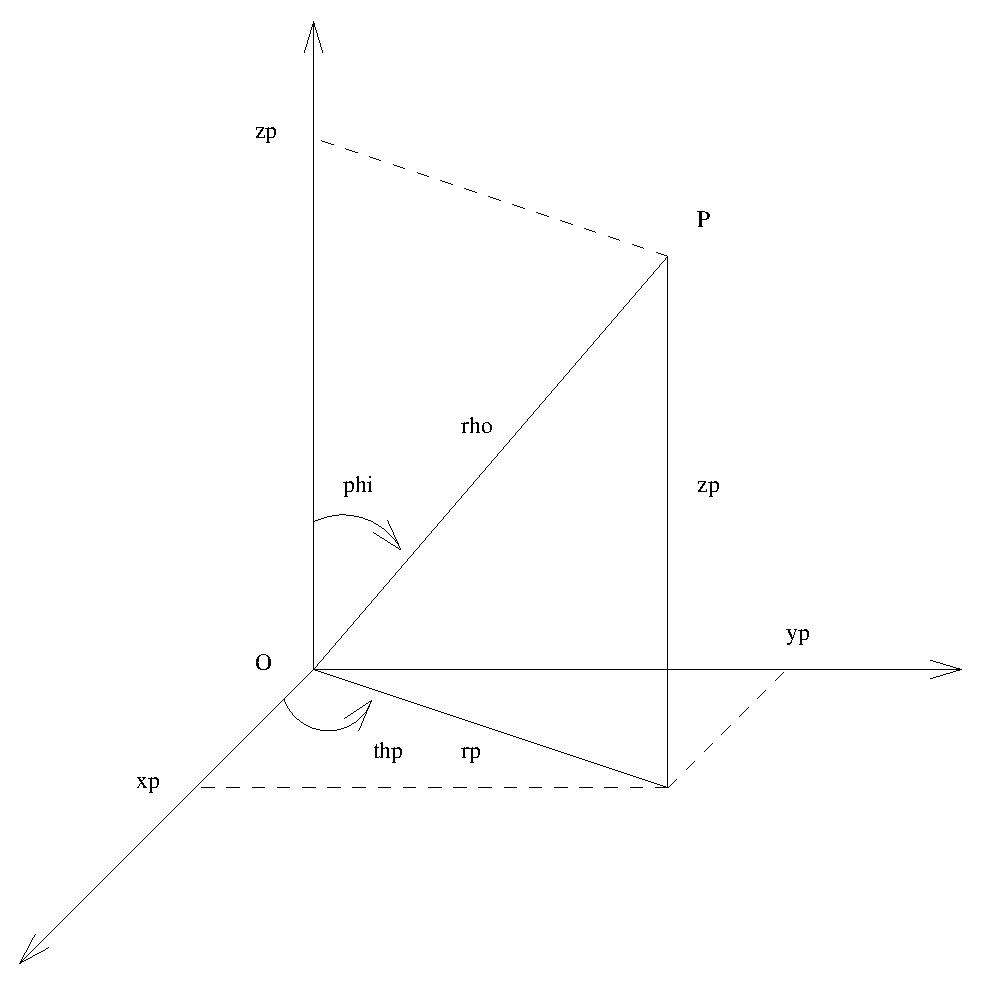
\includegraphics[height=2in]{../../modules/coordinate-systems/pictures/ok-cylindrical-spherical.eps}
\column{0.45\textwidth}
	\begin{itemize}
\item In Cartesian coordinates, a point $P$ is given by triple $(x_P, y_P, z_P)$.
\item<2-> We introduce alternative spherical coordinates $(\rho_P, \phi_P,\theta_P)$.
\begin{itemize}
\item \alert<3>{$\rho_P$: distance $|OP|$;}
\item \alert<4>{$\phi_P$: angle $Oz$ to $OP$;}
\item \alert<5>{$\theta_P$: angle $Ox$ to $OP_{xy}$.}
\end{itemize}
\item<6-> Coordinates range:
\begin{itemize}
\item \alert<7,8>{$\rho$:} \uncover<8->{\alert<8>{ $[0,\infty)$;}}
\item \alert<9,10>{$\phi$:}  \uncover<10->{\alert<10>{$[0, \pi]$;}}
\item \alert<11,12>{$\theta$:}  \uncover<12->{ \alert<12>{$[0,2\pi)$.}}
\end{itemize}
\end{itemize}
\end{columns}
\end{frame}
%\begin{frame}
\frametitle{Spherical curvilinear ``boxes''}


\begin{columns}[T]
\column{0.4\textwidth}

\psset{xunit=1.5cm, yunit=1.5cm}
\begin{pspicture}(-0.6, -0.85)(2.4,1.85)
\tiny
\renewcommand{\fcScreen}{[-5 1 -2.4] 0}
\pstVerb{10 dict begin%
/rhoMin 1 def%
/rhoMax 2 def%
/thetaMin 20 def%
/thetaMax 70 def%
/phiMin 20 def%
/phiMax 70 def%
/xSph {theta cos phi sin rho mul mul} def%
/ySph {theta sin phi sin rho mul mul} def%
/zSph {phi cos rho mul} def%
}%
\fcAxesIIId{2}{2}{2}
\uncover<10->{
\pscustom*[linecolor=pink]{%
\fcCurveIIId{phiMin}{phiMax}{[3 dict begin /rho rhoMin def /phi t def /theta thetaMin def xSph ySph zSph end]}
\fcCurveIIId{rhoMin}{rhoMax}{[3 dict begin /rho t def /phi phiMax def /theta thetaMin def xSph ySph zSph end]}
\fcCurveIIId{thetaMin}{thetaMax}{[3 dict begin /rho rhoMax def /phi phiMax def /theta t def xSph ySph zSph end]}
\fcCurveIIId{phiMax}{phiMin}{[3 dict begin /rho rhoMax def /phi t def /theta thetaMax def xSph ySph zSph end]}
\fcCurveIIId{thetaMax}{thetaMin}{[3 dict begin /rho rhoMax def /phi phiMin def /theta t def xSph ySph zSph end]}
\fcCurveIIId{rhoMax}{rhoMin}{[3 dict begin /rho t def /phi phiMin def /theta thetaMin def xSph ySph zSph end]}
}%
}%
\fcLineIIId[linestyle=dashed]{[0 0 0]}{[0 2 0]}

\uncover<7->{\fcCurveIIId{rhoMin}{rhoMax}{[3 dict begin /rho t def /phi phiMin def /theta thetaMin def xSph ySph zSph end]}}
\uncover<5->{\fcCurveIIId{rhoMin}{rhoMax}{[3 dict begin /rho t def /phi phiMax def /theta thetaMin def xSph ySph zSph end]}}
\uncover<9->{\fcCurveIIId[linestyle=dashed, linecolor=red]{rhoMin}{rhoMax}{[3 dict begin /rho t def /phi phiMin def /theta thetaMax def xSph ySph zSph end]}}
\uncover<9->{\fcCurveIIId[linestyle=dashed, linecolor=red]{rhoMin}{rhoMax}{[3 dict begin /rho t def /phi phiMax def /theta thetaMax def xSph ySph zSph end]}}

\uncover<8->{%
\fcCurveIIId[linestyle=dashed, dash = 2.6pt,  linecolor=red] {thetaMin}{thetaMax}{[3 dict begin /rho rhoMin def /phi phiMin def /theta t def xSph ySph zSph end]}
\fcCurveIIId{thetaMin}{thetaMax}{[3 dict begin /rho rhoMax def /phi phiMin def /theta t def xSph ySph zSph end]}
\fcCurveIIId[linestyle=dashed, linecolor=red]{thetaMin}{thetaMax}{[3 dict begin /rho rhoMin def /phi phiMax def /theta t def xSph ySph zSph end]}
\fcCurveIIId{thetaMin}{thetaMax}{[3 dict begin /rho rhoMax def /phi phiMax def /theta t def xSph ySph zSph end]}
}%

\uncover<4->{\fcCurveIIId{phiMin}{phiMax}{[3 dict begin /rho rhoMin def /phi t def /theta thetaMin def xSph ySph zSph end]}}
\uncover<9->{\fcCurveIIId[linestyle=dashed, linecolor=red]{phiMin}{phiMax}{[3 dict begin /rho rhoMin def /phi t def /theta thetaMax def xSph ySph zSph end]}}
\uncover<6->{\fcCurveIIId{phiMin}{phiMax}{[3 dict begin /rho rhoMax def /phi t def /theta thetaMin def xSph ySph zSph end]}}
\uncover<9->{\fcCurveIIId{phiMin}{phiMax}{[3 dict begin /rho rhoMax def /phi t def /theta thetaMax def xSph ySph zSph end]}}
\pstVerb{end}
\end{pspicture}

\psset{xunit=1cm, yunit=1cm}
\begin{pspicture}(-0.6, -2)(3,2.4)
\tiny
\pstVerb{10 dict begin%
/rhoMin 1 def%
/rhoMax 2 def%
/thetaMin 20 57.2957795 div def%
/thetaMax 70 57.2957795 div  def%
/phiMin 20 57.2957795 div def%
/phiMax 70 57.2957795 div def%
}%
\fcAxesIIId[arrows=->, xLabel=$~~\rho$, yLabel=$~~\phi$, zLabel=$~~\theta$]{2.5}{3.8}{2.5}
\pscustom*[linecolor=cyan]{%
\fcPolyLineIIId{[rhoMin phiMin thetaMin] [rhoMax phiMin thetaMin] [rhoMax phiMax thetaMin] [rhoMax phiMax thetaMax] [rhoMin phiMax thetaMax] [rhoMin phiMin thetaMax] [rhoMin phiMin thetaMin]}
}
\fcLineIIId[linestyle=dashed]{[0 0 0]}{[0 3.8 0]}
\fcDotIIId{[rhoMin 0 0 ]}
\fcPutIIId[t]{[rhoMin 0 -0.2 ]}{$\rho_{min}$}
\fcDotIIId{[rhoMax 0 0 ]}
\fcPutIIId[t]{[rhoMax 0 -0.2 ]}{$\rho_{max}$}
\fcDotIIId{[0 0 thetaMin  ]}
\fcPutIIId[r]{[0 0 thetaMin]}{$\theta_{min}~~$}
\fcDotIIId{[0 0 thetaMax]}
\fcPutIIId[r]{[0 0 thetaMax]}{$\theta_{max}~~$}
\fcDotIIId{[0  phiMin 0  ]}
\fcPutIIId[b]{[0 phiMin 0.2 ]}{$~\phi_{min}$}
\fcDotIIId{[0  phiMax 0  ]}
\fcPutIIId[b]{[0 phiMax 0.2 ]}{$\phi_{max}$}

\fcLineIIId[linecolor=blue, linestyle=dashed]{[rhoMin phiMax thetaMin]}{[rhoMax phiMax thetaMin]}
\uncover<5-9>{\fcLineIIId[linecolor=red, linewidth=2pt, linestyle=dashed]{[rhoMin phiMax thetaMin]}{[rhoMax phiMax thetaMin]}}
\fcLineIIId[linecolor=blue]{[rhoMax phiMax thetaMin]}{[rhoMax phiMin thetaMin]}
\uncover<6-9>{\fcLineIIId[linecolor=red, linewidth=2pt]{[rhoMax phiMax thetaMin]}{[rhoMax phiMin thetaMin]}
}
\fcLineIIId[linecolor=blue]{[rhoMax phiMin thetaMin]}{[rhoMin phiMin thetaMin]}
\uncover<7-9>{\fcLineIIId[linecolor=red, linewidth=2pt]{[rhoMax phiMin thetaMin]}{[rhoMin phiMin thetaMin]}}
\fcLineIIId[linecolor=blue, linestyle=dashed]{[rhoMin phiMin thetaMin]}{[rhoMin phiMax thetaMin]}
\uncover<4-9>{\fcLineIIId[linecolor=red, linewidth=2pt, linestyle=dashed]{[rhoMin phiMin thetaMin]}{[rhoMin phiMax thetaMin]}}

\fcLineIIId[linecolor=blue, linestyle=dashed]{[rhoMin phiMax thetaMax]}{[rhoMin phiMax thetaMin]}
\fcLineIIId[linecolor=blue]{[rhoMax phiMax thetaMax]}{[rhoMax phiMax thetaMin]}
\fcLineIIId[linecolor=blue]{[rhoMax phiMin thetaMax]}{[rhoMax phiMin thetaMin]}
\fcLineIIId[linecolor=blue]{[rhoMin phiMin thetaMax]}{[rhoMin phiMin thetaMin]}
\uncover<8-9>{%
\fcLineIIId[linecolor=red, linestyle=dashed, linewidth=2pt]{[rhoMin phiMax thetaMax]}{[rhoMin phiMax thetaMin]}
\fcLineIIId[linecolor=red, linewidth=2pt]{[rhoMax phiMax thetaMax]}{[rhoMax phiMax thetaMin]}
\fcLineIIId[linecolor=red, linewidth=2pt]{[rhoMax phiMin thetaMax]}{[rhoMax phiMin thetaMin]}
\fcLineIIId[linecolor=red, linewidth=2pt]{[rhoMin phiMin thetaMax]}{[rhoMin phiMin thetaMin]}
}%
\fcLineIIId[linecolor=blue]{[rhoMin phiMax thetaMax]}{[rhoMax phiMax thetaMax]}
\fcLineIIId[linecolor=blue]{[rhoMax phiMax thetaMax]}{[rhoMax phiMin thetaMax]}
\fcLineIIId[linecolor=blue]{[rhoMax phiMin thetaMax]}{[rhoMin phiMin thetaMax]}
\fcLineIIId[linecolor=blue]{[rhoMin phiMin thetaMax]}{[rhoMin phiMax thetaMax]}
\uncover<9>{%
\fcLineIIId[linecolor=red, linewidth=2pt]{[rhoMin phiMax thetaMax]}{[rhoMax phiMax thetaMax]}
\fcLineIIId[linecolor=red, linewidth=2pt]{[rhoMax phiMax thetaMax]}{[rhoMax phiMin thetaMax]}
\fcLineIIId[linecolor=red, linewidth=2pt]{[rhoMax phiMin thetaMax]}{[rhoMin phiMin thetaMax]}
\fcLineIIId[linecolor=red, linewidth=2pt]{[rhoMin phiMin thetaMax]}{[rhoMin phiMax thetaMax]}
}%
\pstVerb{end}
\end{pspicture}

\column{0.6\textwidth}
\begin{itemize}
\item Cut off a rectangular box $B$ in the $\rho, \phi, \theta$-coordinates.
$
B:=\left\{(\rho, \phi, \theta) |\left| \begin{array}{ccccc}
\rho_{min} &\leq& \rho &\leq& \rho_{max} \\
\phi_{min} &\leq& \phi &\leq& \phi_{max}\\
\theta_{min} &\leq& \theta &\leq& \theta_{max}\\
\end{array}\right.\right\}
$
\item<2-> As $(\rho, \phi, \theta)$ traverse $B$, the point $P(\rho, \phi,\theta)$ traverses curvilinear ``box'' $Y$: %in the $x,y,z$-coordinates:
\[
Y = \left\{ P(\rho, \phi, \theta) | (\rho, \phi, \theta)\in B \right\}.
\]
\item<3-> \alertNoH{3-10}{ What is the shape of that curvilinear box?}
\item<11-> What is the volume?
\end{itemize}
\end{columns}
\end{frame}


}
\end{document}
